
%%% Uncomment for slide version
\documentclass[xcolor=dvipsnames]{beamer}
\setbeameroption{hide notes} % Only slides

%%% Uncomment for handout version
%\documentclass[handout]{beamer}
%\setbeameroption{show notes on second screen=right} % Both

\usepackage{enumitem}
\usepackage{listings}
\usepackage{adjustbox} % To incorporate code into Latex
\usepackage{multirow} % To merge multiple rows  in a table
\usepackage{soul} % To put in strikethrough text
\usepackage{array}
\usepackage{makecell}

\setbeamertemplate{note page}{\pagecolor{white}\insertnote}
\setbeamertemplate{footline}{}
\usetheme[progressbar=frametitle]{moloch}% modern fork of the metropolis theme
\setbeamercolor{background canvas}{bg=white}
\setbeamercolor{frametitle}{fg=black,bg=ProcessBlue!20}

\setbeamercolor{progress bar}{use=palette primary,fg=black,bg=black}
\setbeamercolor{note page}{bg=white} 
\setbeamertemplate{date}{}


\DeclareUnicodeCharacter{0313}{*************************************}

\setbeamertemplate{page number in head/foot}{}


\addtobeamertemplate{navigation symbols}{}{%
	\usebeamerfont{footline}%
	\usebeamercolor[fg]{footline}%
	\hspace{1em}%
	\insertframenumber/\inserttotalframenumber
}
\setbeamercolor{itemize item}{fg=black}
\setbeamercolor{itemize subitem}{fg=black}
\setbeamercolor{itemize subsubitem}{fg=black}

\newcommand\blfootnote[1]{%
	\begingroup
	\renewcommand\thefootnote{}\footnote{#1}%
	\addtocounter{footnote}{-1}%
	\endgroup
}

%%%%%%%%%%%%%%%%%%
%%%%%%%%%%%%%%%%%%
%%%%%%%%%%%%%%%%%%
%%%%%%%%%%%%%%%%%%
%%%%%%%%%%%%%%%%%%
%%%%%%%%%%%%%%%%%%
%%%%%%%%%%%%%%%%%%




\title{\Huge FRST302: Forest Genetics}
\author{\Large Lecture 4.1 -  Accelerating Tree Improvement II}
\date{\today}

\begin{document}
	\maketitle
	
	\begin{frame}
\frametitle{Recap}
\begin{itemize}
	\item There are numerous ways to suvey genetic markers at scale (e.g. WGS, reduced representation sequncing, SNP-chips)
	\item Association genetics is a powerful way to identify genes underlying important traits
	\item Association genetics \textbf{is not} a silver bullet as there are multiple statistical issues
	\item Good at identifying large effect loci
	
\end{itemize}

\end{frame}



\begin{frame}
	
\frametitle{Now What?}
	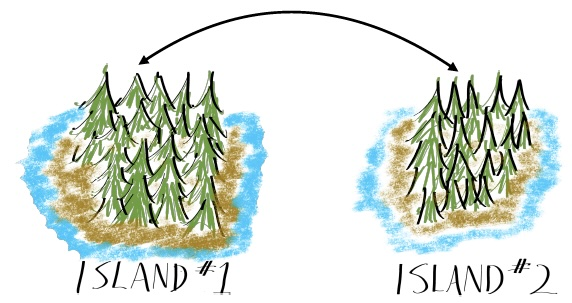
\includegraphics[keepaspectratio, width  = 0.7\textwidth]{img/treeIslands}
				
\end{frame}


	
\end{document}


%%%
\begin{columns}
	\begin{column}{0.5\textwidth}
	\end{column}
	\begin{column}{0.5\textwidth}
	\end{column}
\end{columns}



